\begin{figure}
    \centering
    % 
\includegraphics[scale=0.6]{pictures/qualitative-row-1}
    % 
\includegraphics[scale=0.6]{pictures/qualitative-row-2}
    % 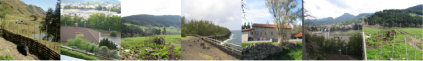
\includegraphics[scale=0.6]{pictures/qualitative-row-5}
    % 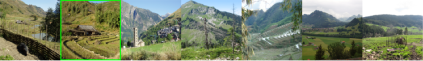
\includegraphics[scale=0.6]{pictures/qualitative-row-6}
    % 
\includegraphics[scale=0.6]{pictures/qualitative-row-7}
    % 
\includegraphics[scale=0.6]{pictures/qualitative-row-8}
    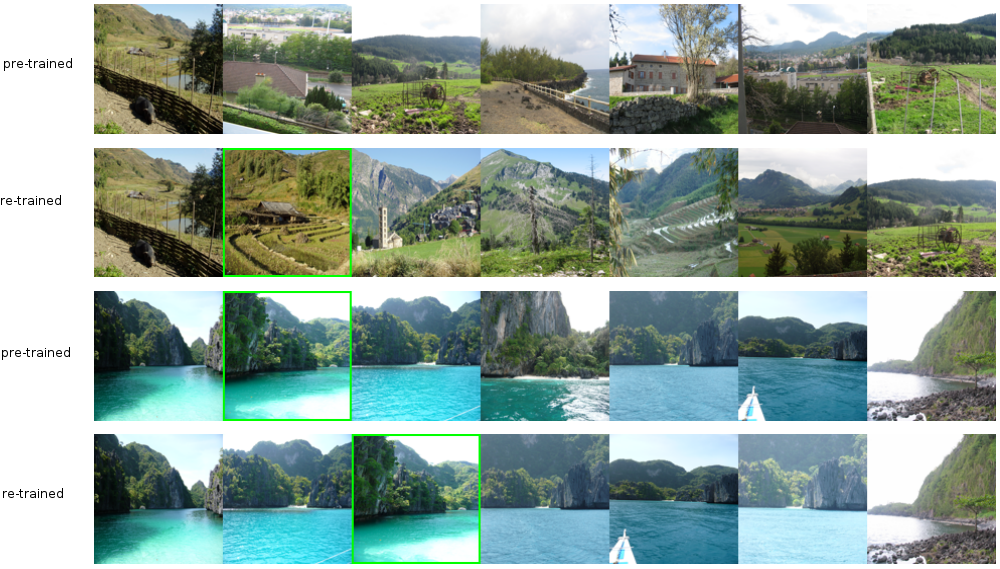
\includegraphics[scale=0.4]{pictures/qualitative-annotated}
    \caption{Two retrieval examples (taken from \cite{BabenkoSlesarevChigorinLempitsky:2014}) on the Holidays dataset using the pre-trained model (on the top, respectively) and the re-trained model (on the bottom, respectively). In each row, the left-most image is the query image and correctly retrieved images are outlined in green. Babenko \etal point out that the lower example is a ``rare exception'' \cite[p. 10]{BabenkoSlesarevChigorinLempitsky:2014} where the pre-trained model outperforms the re-trained model.}
    \label{fig:qualitative}
\end{figure}

\section{Conclusion}
\label{sec:conclusion}

In the course of this report we presented current techniques in content-based image retrieval. In particular, we discussed local descriptors and their aggregation techniques in Section \ref{subsubsec:local-descriptors}, as well as global descriptors in Section \ref{subsubsec:global-descriptors}. Furthermore, after discussing convolutional neural networks in Section \ref{sec:convolutional-neural-networks}, we discussed the use of convolutional neural networks in image retrieval in Section \ref{sec:neural-codes-image-retrieval}. Finally, we presented experimental results following Babenko \etal \cite{BabenkoSlesarevChigorinLempitsky:2014} in Section \ref{sec:experiments}.

Overall, we discussed many approaches related to the Bag of Visual Words model \cite{SivicZisserman:2003} relying mostly on hand-crafted descriptors. Although some techniques make use of metric learning or similar (supervised or unsupervised) learning techniques, the embedding step and/or the aggregation step are heavily guided by manual processes, that is the whole retrieval system is explicitly engineered by hand.
% This includes all subproblems discussed in Section \ref{sec:image-retrieval}: local descriptors, normalization, embedding and aggregation.
In strong contrast, Babenko \etal use convolutional neural networks to automatically learn most of these tasks. Although, the presented results are not fully convincing, especially on the Oxford 5k dataset \cite{PhilbinChumIsardSivicZisserman:2007}, this approach opens a new direction of research where several subproblems are solved fully by learning algorithms. Still, the image retrieval community will try to improve these results by adapting pre- or post-processing as well as network architecture.

\subsection{Research Questions}

We conclude that combining hand-crafted approaches with convolutional neural networks may be a promising future research direction. For example, different normalization techniques (for example \cite{ArandjelovicZisserman:2013}) may improve performance. Furthermore, layer selection has only be done experimentally based on the mean average precision. In contrast, visualizing the energy of the image representations as done in \cite{ArandjelovicZisserman:2013} may help to select suitable layers. In addition, the convolutional neural network was explicitly trained in a classification framework. Other architectures, as for example a Siamese architecture (see \cite{BabenkoSlesarevChigorinLempitsky:2014} for references), may be tailored directly towards the image retrieval task. Finally, techniques allowing to combine the information of multiple layers similar to \cite{GeKeSun:2013} may be interesting.
